\documentclass[10pt]{article}
\usepackage[margin=0.78in]{geometry}
\usepackage{graphicx,booktabs,microtype,xcolor,amsmath,float}
\usepackage[colorlinks=true,allcolors=blue!55!black]{hyperref}
\makeatletter
\renewcommand\section{\@startsection{section}{1}{0pt}{7pt}{3pt}{\normalfont\bfseries}}
\makeatother
\setlength{\parskip}{1pt}
\setlength{\parindent}{12pt}
\pagestyle{empty}

\title{\vspace{-2.2em}\textbf{Do agent routers need to look inside the model?}\\[-0.1em]
\large A preliminary audit of internal-state failure probes}
\author{Shlok Channawar}
\date{\vspace{-1em}\small September 2026}

\begin{document}
\maketitle
\vspace{-1.6em}

\section{Motivation}

\href{https://arxiv.org/abs/2605.24598}{Hera},
\href{https://aclanthology.org/2026.acl-long.2045/}{MTRouter} and CEB all need an
estimate of the acting model's state \emph{at each step} in order to route or
intervene, and all three reconstruct it from outside the
model. Hera observes that device/cloud step agreement correlates with predictive
entropy---an internal signal---then trains a separate 500M network to read state text
instead. MTRouter cannot inspect a mostly-closed model pool, so it learns a per-model
residual vector as a proxy for behavioural character it cannot observe. CEB keeps the
model frozen and routes through what it can articulate; its Appendix~F reports TF-IDF
beating dense embeddings, because the retrieval target is near-duplicate actions on
near-identical pages. Three workarounds for one missing measurement.

\textbf{Does that signal exist inside the acting model at each step, is it richer than
entropy, and does it generalise along failure \emph{structure} rather than surface
similarity?} Ruan et al.~(\href{https://arxiv.org/abs/2607.06503}{2607.06503}) is the
one paper here that reads hidden states directly: AUC~$0.81$ for predicting eventual
failure from a layer-28 state at the final token of the agent's first action
(TextCraft, Qwen3-1.7B), used to gate an abort cascade. If it means what it appears
to, it is the measurement the other three approximate.

\section{Preliminary experiment: does the reported metric measure step-level state?}

Any per-step decision requires knowing that \emph{this rollout} is going wrong, not
that \emph{this task} is hard. Ruan's reported statistic is a pooled cross-fitted
AUC over all episodes, which cannot separate these: a probe that only reads task
difficulty scores well on it while carrying no per-rollout information at all.

We replicated the TextCraft/Qwen3-1.7B cell (1000 episodes; 125 depth-one tasks
$\times$ 8 rollouts; 20-round cap; L2 logistic probe, $C{=}1$; task-grouped
stratified cross-fitting) and obtained \textbf{pooled AUC 0.791} against their 0.81.
We then added the control the paper does not report: \textbf{within-task AUC}, which
compares failures against successes \emph{on the same task}, so task difficulty is
held constant by construction.

\begin{center}\small
\begin{tabular}{lcc}
\toprule
& pooled AUC & within-task AUC \\
\midrule
Hidden state, layer 28 (reported config) & 0.791 & \textbf{0.547} \\
Five cheap surface features & 0.698 & 0.615 \\
TF-IDF text + surface & 0.717 & 0.606 \\
\bottomrule
\end{tabular}
\end{center}

\textbf{99.6\% of the comparisons behind the pooled number are between different
tasks} (173{,}748 of 174{,}375); only 627 hold the task fixed. 77\% of score variance
is between tasks: the probe emits approximately one score per task
(Fig.~\ref{fig:one}). Held to the same task, it falls to chance, and the cheap
surface baseline beats it.

\begin{figure}[H]\centering\vspace{-2pt}
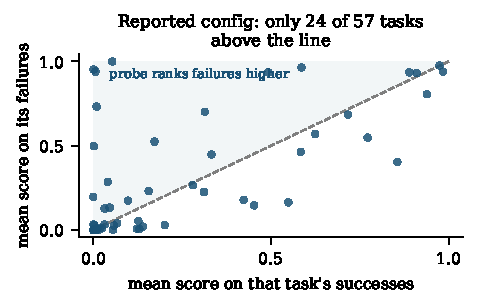
\includegraphics[width=0.45\textwidth]{fig1_confound.pdf}\hfill
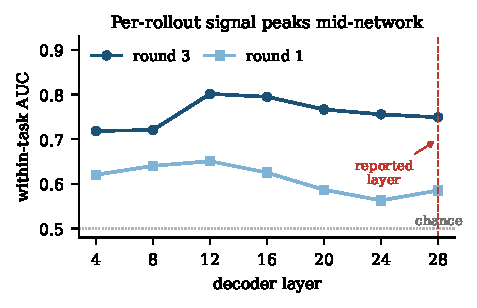
\includegraphics[width=0.45\textwidth]{fig2_layers.pdf}
\caption{\small \textbf{Left:} for each mixed-outcome task, mean probe score on its
failures against its successes. A probe carrying within-task information would sit
above the dashed diagonal; only 24 of 57 tasks do. \textbf{Right:} within-task AUC by layer.
The reported layer sits on the downslope; layer 12 wins at both rounds, and at round 1
it wins on the paper's own selection criterion (pooled AUC 0.830 vs 0.781).}
\label{fig:one}\vspace{-6pt}
\end{figure}

\vspace{-0.6em}
\section{What the probe was actually detecting}

Classifying all 225 failures by behaviour makes this concrete. At the reported
configuration the probe catches \textbf{77\%} of failures on tasks whose recipe names
a count-one plural ingredient (\texttt{craft 4 acacia planks using 1 acacia logs}:
the plural form is a distinct item and the model silently ``corrects'' it) and
\textbf{29\%} of every other failure. It is largely a detector for one lexical
quirk---the same surface-similarity behaviour that motivates the concern about CEB's
TF-IDF retrieval.

\section{The signal exists, but not at the reported coordinates}

Sweeping rounds $1$--$6$ and layers $\{4,8,\dots,28\}$ (each layer captured in one
forward pass) locates it elsewhere. At \textbf{layer 12, round 3}, within-task AUC
reaches \textbf{0.801} (95\% CI $[0.74,0.86]$), against 0.749 at layer 28 and
\textbf{0.725} for a text model given every prompt, response and error message
through round 3. Detection also generalises: looping rises from $\sim$29\% to 73\%
across 213 episodes, format errors to 80\%, explicit give-ups to 83\%
(Fig.~\ref{fig:two}), while eventual successes stay at 0.195.

\begin{figure}[H]\centering\vspace{-2pt}
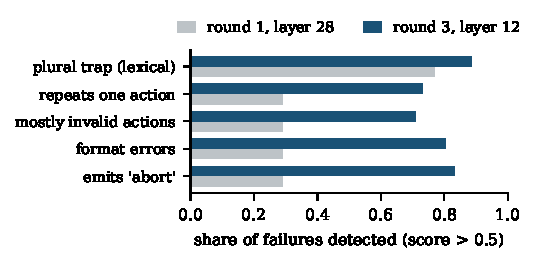
\includegraphics[width=0.5\textwidth]{fig3_modes.pdf}
\caption{\small Detection by failure mode: from one lexical quirk to failure
structure. The reported configuration finds the lexical trap; the better-placed probe
finds failure shapes that share no vocabulary.}
\label{fig:two}\vspace{-6pt}
\end{figure}

\vspace{-0.6em}
\section{Opportunity, and what would falsify this}

The three sub-questions have provisional answers: the signal \emph{does} exist per
step, is modestly richer than entropy-like surface features, and generalises along
failure structure rather than surface similarity---but only at a readout point the
literature does not report, and the reported configuration is precisely the one at
which the answer looks negative.

\textbf{Scope.} This audits Ruan's evaluation methodology. We have not tested whether
Hera's agreement signal or MTRouter's outcome estimator conflate difficulty with
instance; they are motivating contrast, not targets of critique.

\textbf{Limits.} Layer 12 / round 3 is a cell selected from a $7\times6$ search, so
0.801 is an exploratory maximum, not an effect size. Sweeps ran on MPS against CUDA
canonical features (0.547 vs 0.585 at the same cell). The text baseline is TF-IDF, a
weak stand-in for an LLM judge. One environment, one 1.7B model, and ``failure''
means the item was not crafted, not that an unsafe action was taken.

\textbf{Next, ranked.} (i) An LLM-as-judge baseline---the comparison that decides
whether internals are worth instrumenting at all. (ii) A pre-registered replication
with layer 12 / round 3 fixed in advance on a fresh seed. (iii) A paired fold-level
test rather than overlapping intervals. (iv) The same decomposition where the label
is an unsafe action rather than a failed task, which is what would make this safety
work rather than reliability work.

\end{document}
